\section{lib/efreet\_\-trash.c File Reference}
\label{efreet__trash_8c}\index{lib/efreet\_\-trash.c@{lib/efreet\_\-trash.c}}


{\tt \#include $<$errno.h$>$}\par
{\tt \#include $<$time.h$>$}\par
{\tt \#include \char`\"{}Efreet.h\char`\"{}}\par
{\tt \#include \char`\"{}Efreet\_\-Trash.h\char`\"{}}\par
{\tt \#include \char`\"{}efreet\_\-private.h\char`\"{}}\par


Include dependency graph for efreet\_\-trash.c:\nopagebreak
\begin{figure}[H]
\begin{center}
\leavevmode
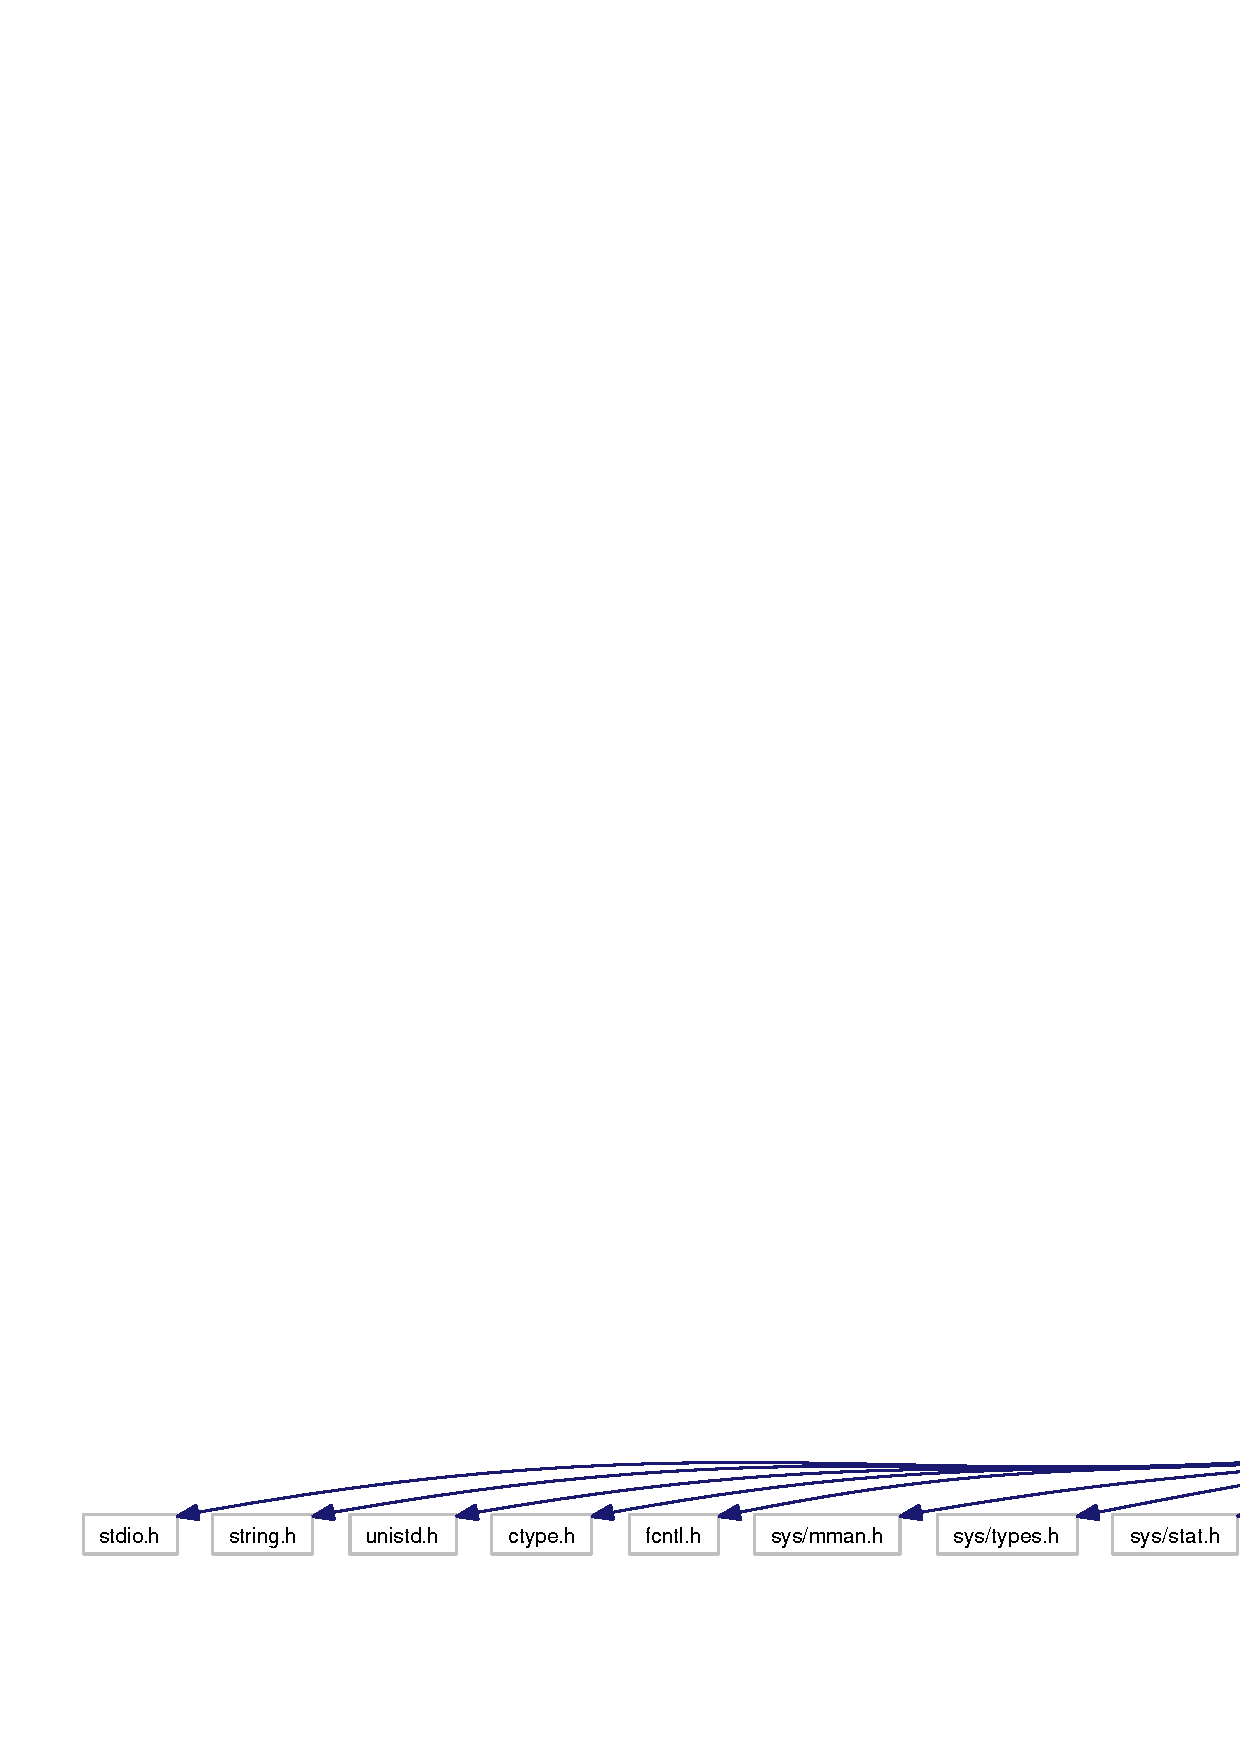
\includegraphics[width=420pt]{efreet__trash_8c__incl}
\end{center}
\end{figure}
\subsection*{Functions}
\begin{CompactItemize}
\item 
EAPI int {\bf efreet\_\-trash\_\-delete\_\-uri} ({\bf Efreet\_\-Uri} $\ast$uri, int force\_\-delete)
\begin{CompactList}\small\item\em This function try to move the given uri to the trash. Files on different filesystem can't be moved to trash. If force\_\-delete is 0 than non-local files will be ignored and -1 is returned, if you set force\_\-delete to 1 non-local files will be deleted without asking. \item\end{CompactList}\item 
EAPI const char $\ast$ {\bf efreet\_\-trash\_\-dir\_\-get} (void)
\begin{CompactList}\small\item\em Retrieves the XDG Trash local directory. \item\end{CompactList}\item 
EAPI int {\bf efreet\_\-trash\_\-empty\_\-trash} (void)
\begin{CompactList}\small\item\em Delete all the files inside the trash. \item\end{CompactList}\item 
EAPI int {\bf efreet\_\-trash\_\-init} (void)
\begin{CompactList}\small\item\em Initializes the efreet trash system. \item\end{CompactList}\item 
EAPI int {\bf efreet\_\-trash\_\-is\_\-empty} (void)
\begin{CompactList}\small\item\em Check if the trash is currently empty. \item\end{CompactList}\item 
EAPI Ecore\_\-List $\ast$ {\bf efreet\_\-trash\_\-ls} (void)
\begin{CompactList}\small\item\em List all the files and directory currently inside the trash. \item\end{CompactList}\item 
EAPI void {\bf efreet\_\-trash\_\-shutdown} (void)
\begin{CompactList}\small\item\em Cleans up the efreet trash system. \item\end{CompactList}\end{CompactItemize}
